\documentclass[11p]{article}
% Packages
\usepackage{amsmath}
\usepackage{graphicx}
\usepackage[swedish]{babel}
\usepackage[
    backend=biber,
    style=authoryear-ibid,
    sorting=ynt
]{biblatex}
\usepackage[utf8]{inputenc}
\usepackage[T1]{fontenc}
%Källor

\graphicspath{ {./images/} }

\title{Labrapprt \\ \small Fysik 1}
\author{Magnus Silverdal }
\date{\today}

\begin{document}

    \begin{titlepage}
        \begin{center}
            \vspace*{1cm}

            \Huge
            \textbf{Laboration El}

            \vspace{0.5cm}
            \LARGE
            Ellära

            \vspace{1.5cm}

            \textbf{Ditt namn!}

            \vfill


            Fysik 1

            \vspace{0.8cm}

            
\includegraphics[width=0.4\textwidth]{../images/NTI Gymnasiet_Symbol_print_svart.png}

            \Large
            Teknikprogrammet\\
            NTI Gymnasiet\\
            Umeå\\
            \today

        \end{center}
    \end{titlepage}
    \section{Syfte och frågeställning}
    \section{Del 1}
    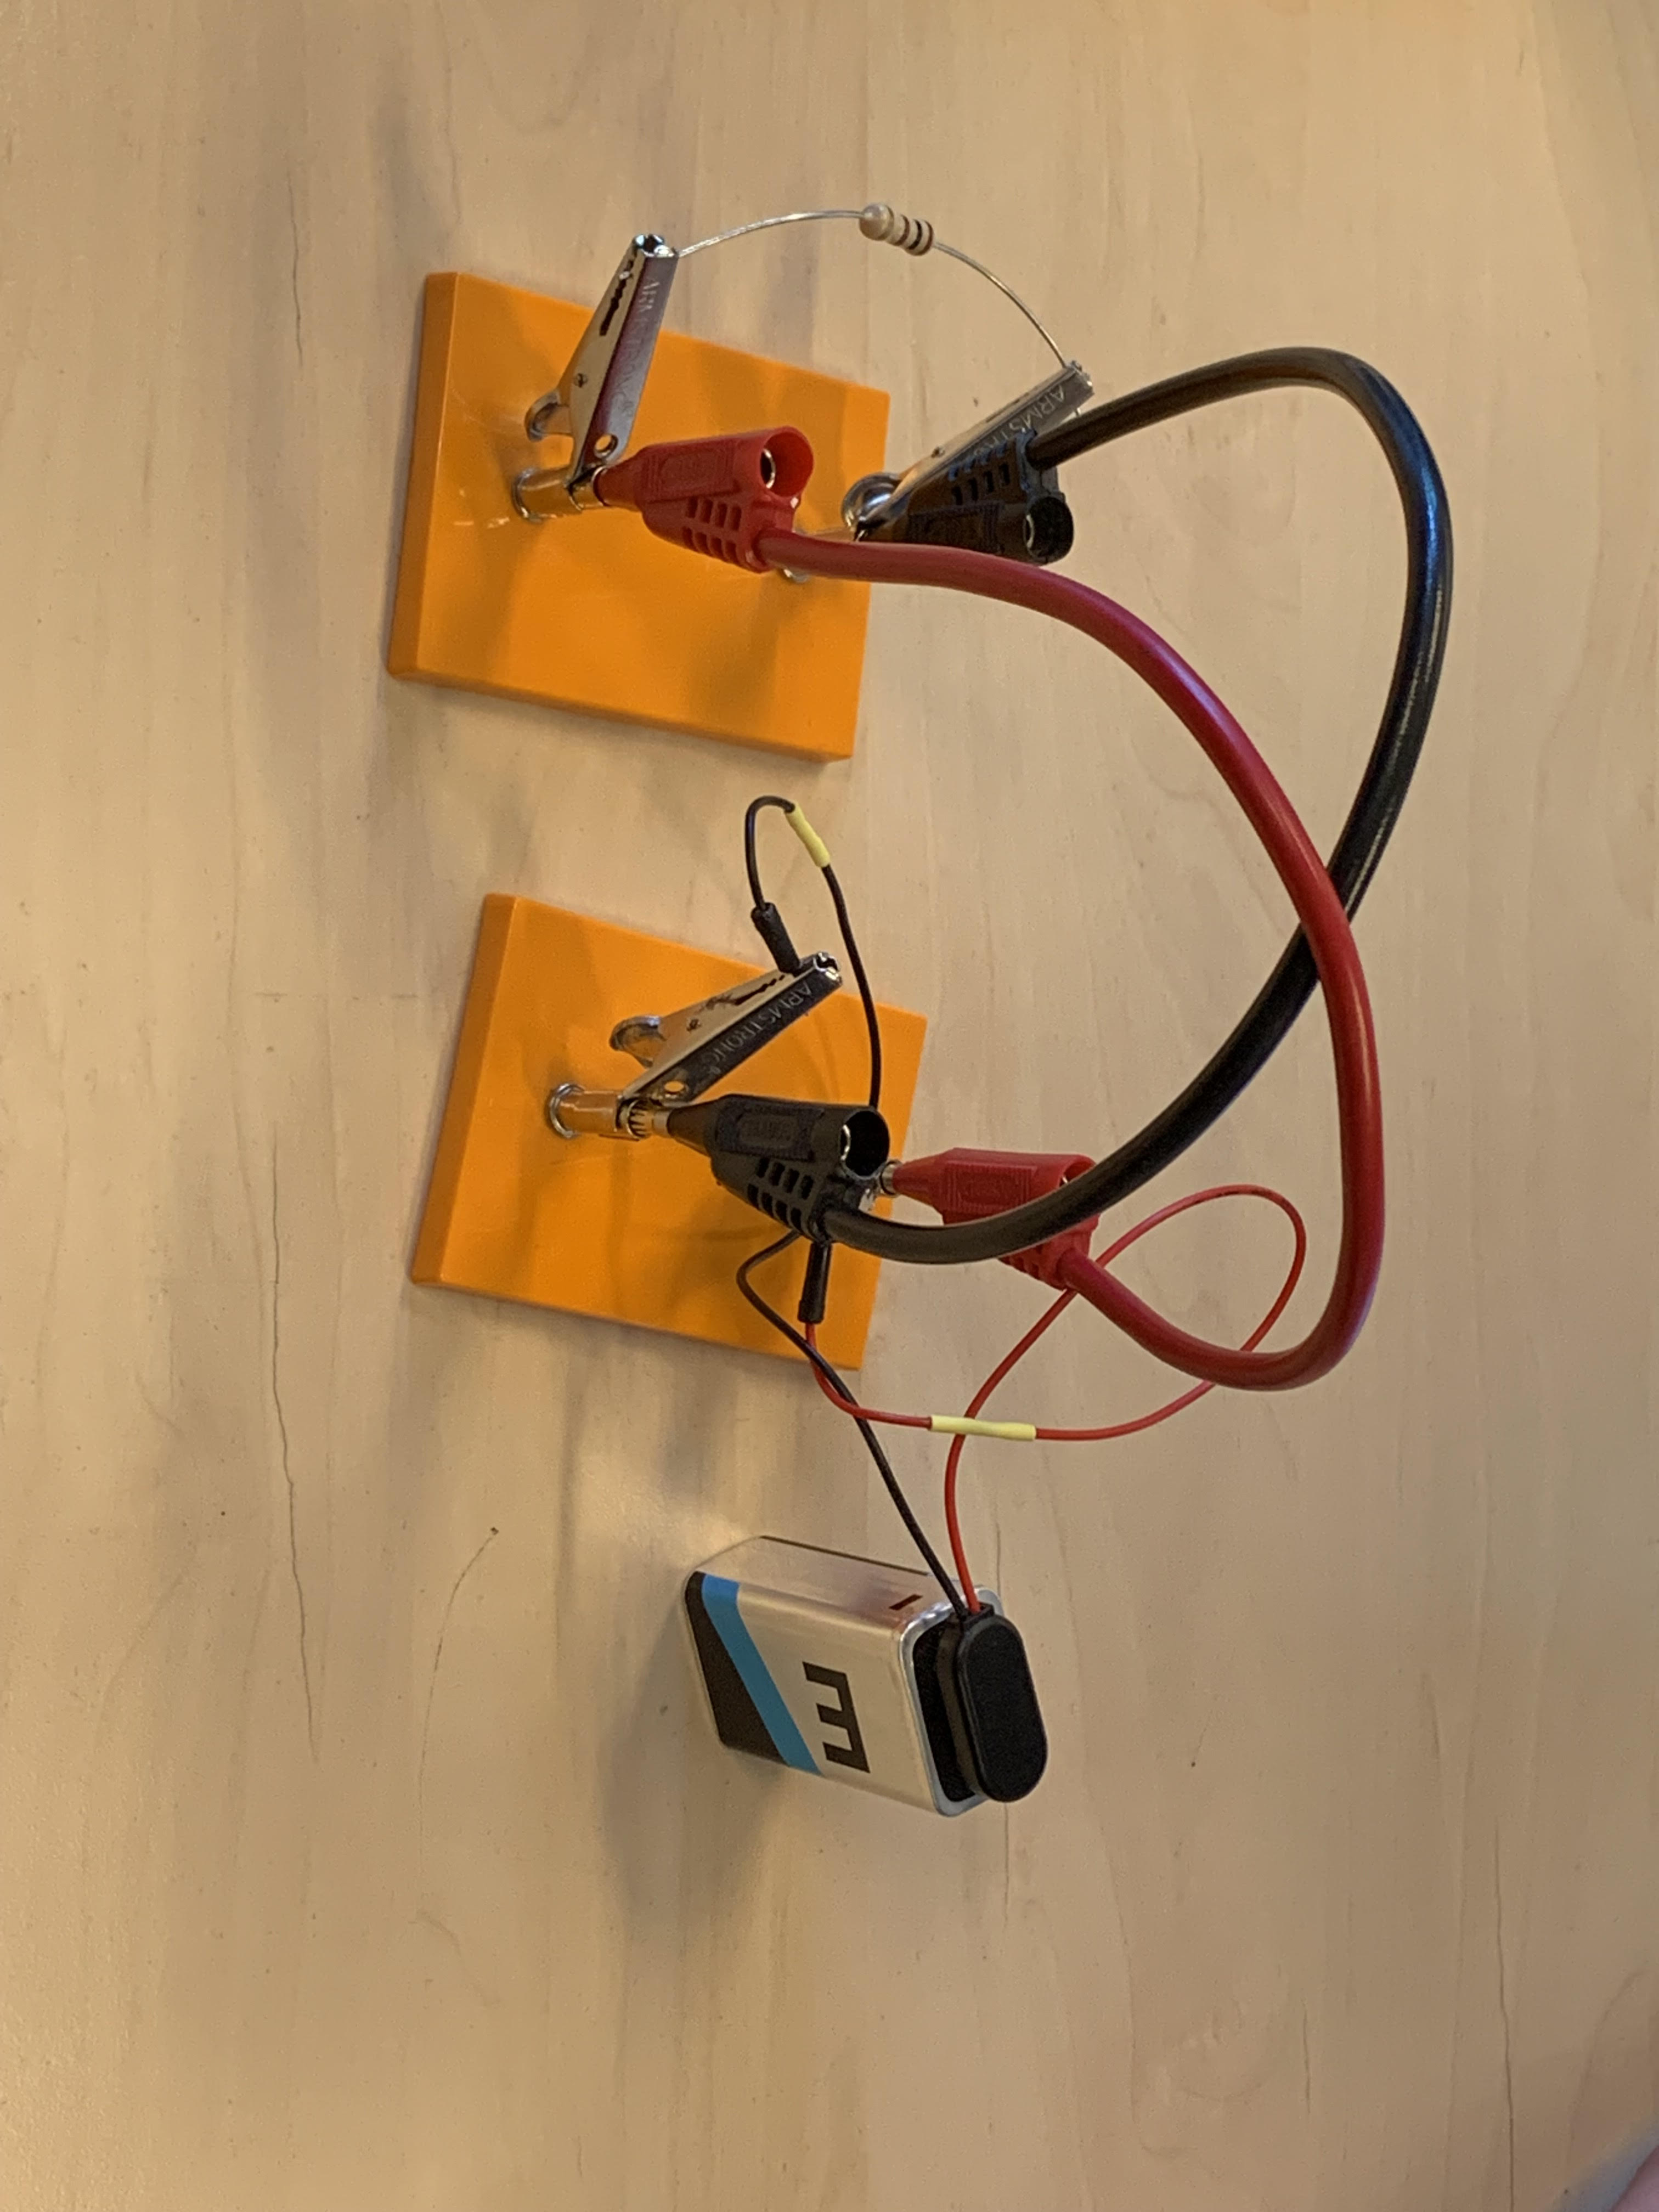
\includegraphics[width=0.4\textwidth]{../images/Elbild.jpg}
    \subsection{Material och metod}
    9V batteri, kablar,  multimeter, kopplingsutrustning och motstånd
    Vi skapade en krets med en resistor och mätte strömmen i Ampere och spänningen i Volt med multimetern.
    På bilden så ser vi hur batteriet är kopplat för att kunna skapa en fungerande krets.
    \subsection{Resultat}
    Vi fick att strömmen var 0,08A och att spänningen var 9V. Resistansen blev 112,5 ohm.
    \subsection{Analys}
    För att få ut resistansen så delar man spänningen med strömmen
    \begin{equation} R = \frac{9}{0,08}\end{equation}
    och 9 delat på 0,08 är 112,5. Alltså är resistansen 112,5 ohm.
    \section{Del 2}
    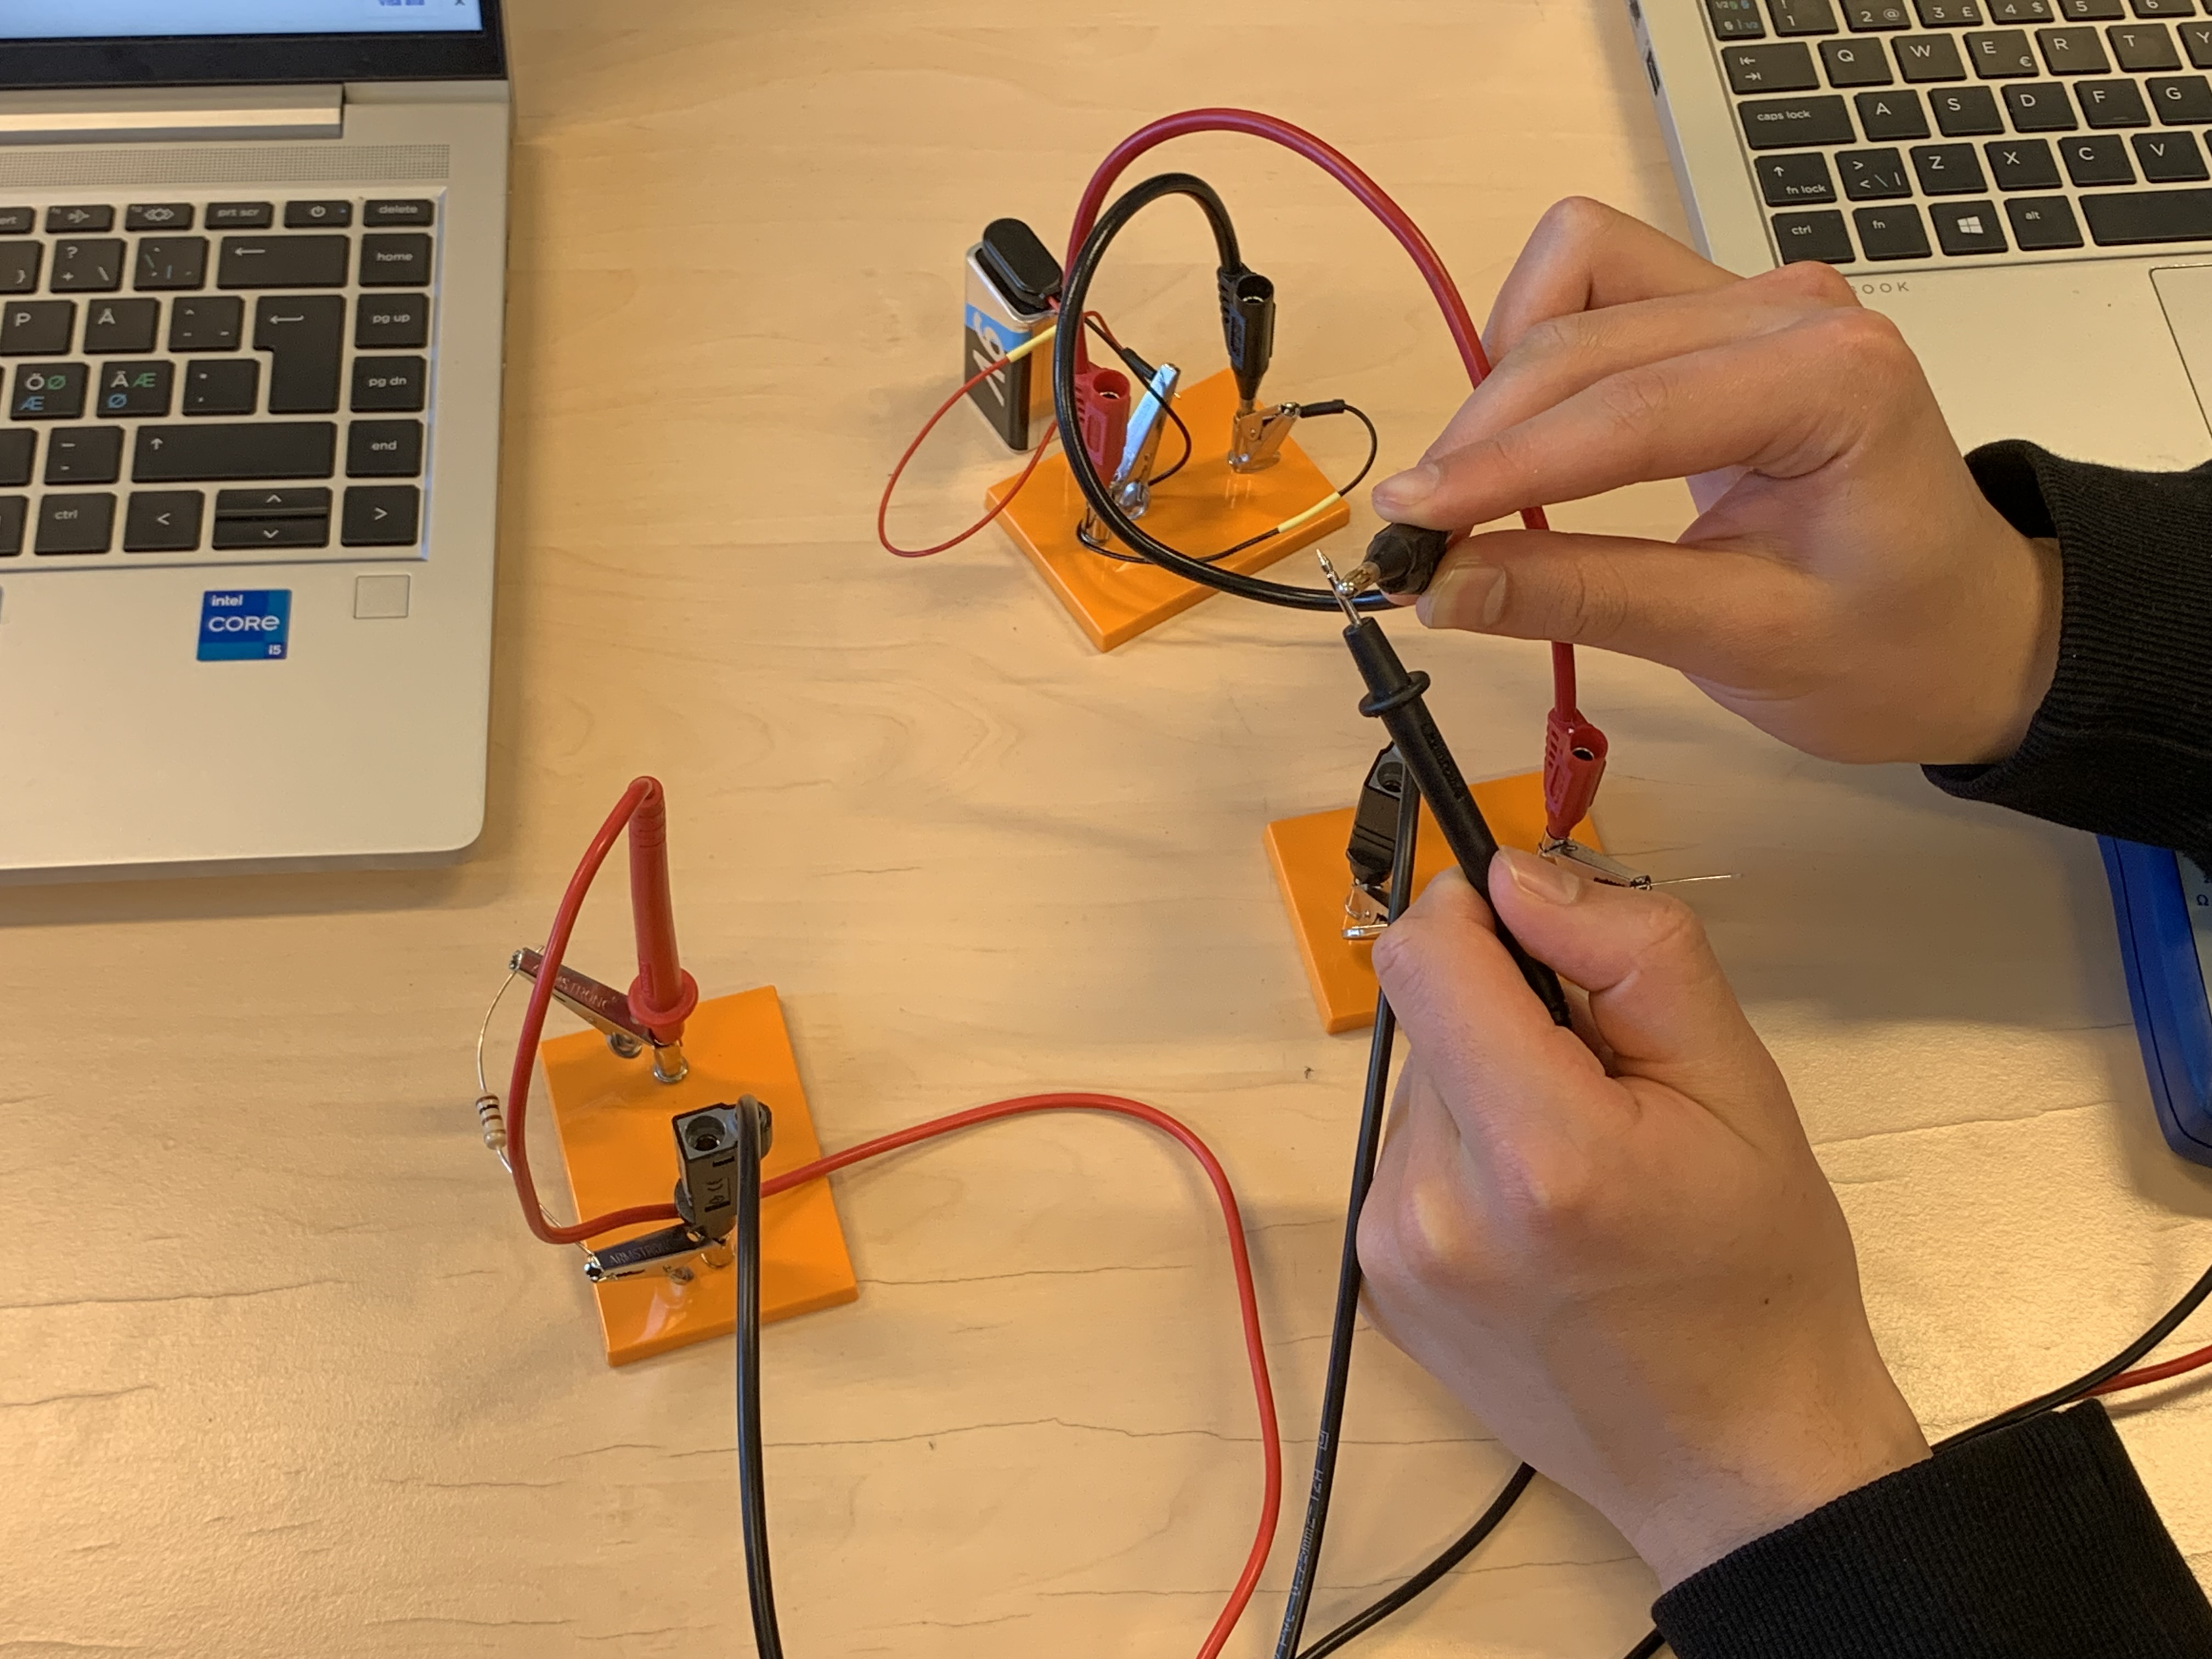
\includegraphics[width=0.4\textwidth]{../images/Elbild2.jpg}
    \subsection{Material och metod}
Vi skapade en krets där vi seriekopplade två styckna resistorer och mätte spänning och ström över en av resistorena.
    Man ser på bilden att resistorerna är seriekopplade för dom är kopplade i rad istället för parallell koppling för då hade de varit kopplade sida vid sida.
    \subsection{Resultat}
    Spänningen över en av resistorn var 4,05V och strömmen var 0,04 A
    \subsection{Analys}
    Teknist sätt så borde vi fått en spänning på 4,5V för \begin{equation} U = 112,5 * 0,04 \end{equation} och strömmen borde teknist sätt varit 0,036A för \begin{equation} R = \frac{4,05}{112,5}\end{equation}
Så siffrorna vi fick stämde icke överens med vetenskapen dock så var siffrorna vi fick väldigt nära intill på vad dom borde varit så det uppstod antagligen ett lite fel någonstans i vår process.
    \section{Diskussion}
\end{document}
